\documentclass[english,11pt,a4paper,titlepage]{report}
\usepackage[T1]{fontenc}
\usepackage{babel, graphicx, amsmath, indentfirst}
\title{Hand-in 1}
\author{Rasmus Freund}
\begin{document}
	\maketitle
	
	\section*{Part I: Logistic Regression}
	\subsection*{Code}
	\subsubsection*{Summary and Results}
	
	\begin{figure}[h]
		\centering
		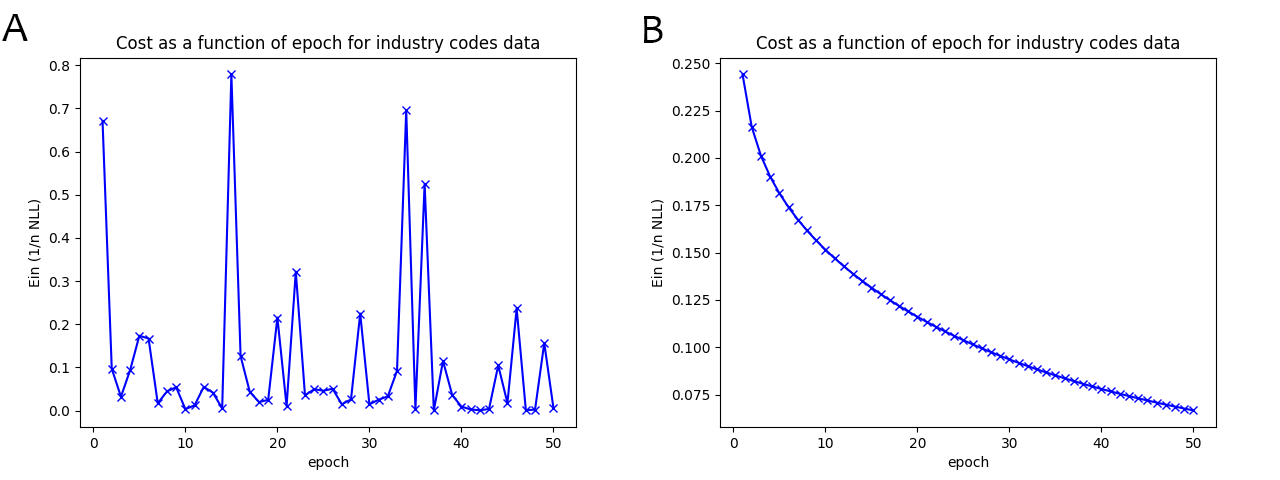
\includegraphics[width=0.9\linewidth]{h1git/results/logreg_text_cost_per_epoch_combined}
		\caption{A: cost function when randomly permuting data before each epoch B: cost function without random permutation}
		\label{fig:logregtextcostperepochcombined}
	\end{figure}
	
	\begin{table}[h]
	\begin{tabular}{rll}
							& In-sample accuracy 	& Test accuracy 		\\
		No permutation 		& 0.9743068391866914	& 0.9672949002217295	\\
		With permutation	& 0.9761552680221811	& 0.9611973392461197
		
	\end{tabular}
	\end{table}
		
		Plot A shows erratic behaviour of the loss function - this appears to be the result of permuting the data before running every epoch, as this behaviour disappears when permutations aren't used.
	
	\subsubsection{Actual Code}
		
		\begin{verbatim}
			def cost_grad(self, X, y, w):
				cost = 0
				grad = np.zeros(w.shape)
				### YOUR CODE HERE
				n = X.shape[0]
				cost = -np.mean(np.log(1 / (1 + np.exp(-y * np.dot(X, w)))))
				
				z = y * np.dot(X, w)
				sigmoid_z = logistic(z)
				grad = -(1/n) * np.dot(X.T, y * (1 - sigmoid_z))
				
				### END CODE
				assert grad.shape == w.shape
				return cost, grad
		\end{verbatim}
		
		\begin{verbatim}
			def fit(self, X, y, w=None, lr=0.1, batch_size=16, epochs=10):
			if w is None:
				w = np.zeros(X.shape[1])
			cost = 0
			history = []
			### YOUR CODE HERE
			for epoch in range(epochs):
			    permutation = np.random.permutation(X.shape[0])
			    X = X[permutation]
			    y = y[permutation]
			    for i in range(0, X.shape[0], batch_size):
			        X_batch = X[i: i + batch_size]
			        y_batch = y[i: i + batch_size]
			
			        # Compute cost and gradient
			        cost, grad = self.cost_grad(X_batch, y_batch, w)
			
			        # Update weights using gradient descent
			        w -= lr * grad
			
			    avg_cost = np.mean(cost)
			    history.append(avg_cost)
			
			    print(f"Epoch {epoch + 1}/{epochs}, Avg. cost: {avg_cost}")
			
			### END CODE
			self.w = w
			self.history = history
		\end{verbatim}
		
	\subsection*{Theory}
	
	1. What is the running time of your mini-batch gradient descent algorithm?\\
	
	Assuming that permuting the data set takes $O(n * log(n))$:
		
	\begin{align*}
		O&(\textrm{epochs} * (n * log(n) + \frac{n}{mini\_batch\_size} * mini\_batch\_size * d))) \\
		= & \ O(\textrm{epochs} * (n * log(n) + n * d))
	\end{align*}
	
	\pagebreak
	
	2. Assume you are using Logistic Regression for classifying images of cats and dogs. What happens if we randomly permute the pixels in each image (with the same permutation) before we train the classifier? Will we get a classifier that is better, worse, or the same than if we used the raw data?
	\\
	
	I would expect a (much) worse classifier. Permutation of an image destroys the information regarding locality. Just like many other image classifiers, a logistic regression model relies on the relationship between neighbouring pixels for classification. \\
	
	3. If the data is linearly separable, what happens to weights when we implement logistic regression with gradient descent?
	\\
	
	Given linearly separable data, weights will tend towards infinity because the model will attempt to locate a decision boundary that maximizes the likelihood of the data. If the data is linearly separable, increasing the weights will \textit{always} increase the likelihood, meaning that we will never find an optimum.
	
	\section*{Part II: Softmax}
	\subsection*{Code}
	\subsubsection{Summary and Results}
	
	\subsubsection{Actual code}
	
	\subsection*{Theory}	
	
	
	
	
	
\end{document}